\chapter{Figures}
\label{chap:figures}

\section{Including an image}

Put image files (PNG, JPG or PDF) in the \texttt{images/} folder and include
them by name, without the extension. \Cref{fig:single} is
\texttt{images/example-figure.png}.

\begin{figure}[H]
  \centering
  
\includegraphics[width=0.7\linewidth]{example-figure}
  \caption{An image included with \texttt{\textbackslash includegraphics}.}
  \label{fig:single}
\end{figure}

\section{Subfigures}

Several images can share one figure number and get their own letter, as in
\cref{fig:sub-a,fig:sub-b}, which are both parts of \cref{fig:subfigures}.

\begin{figure}[H]
  \centering
  \begin{subfigure}[b]{0.48\linewidth}
    \centering
    
\includegraphics[height=3.6cm]{example-figure}
    \caption{First view.}
    \label{fig:sub-a}
  \end{subfigure}
  \hfill
  \begin{subfigure}[b]{0.48\linewidth}
    \centering
    
\includegraphics[height=3.6cm, trim=0 0 200 0, clip]{example-figure}
    \caption{Cropped with \texttt{trim} and \texttt{clip}.}
    \label{fig:sub-b}
  \end{subfigure}
  \caption{Two subfigures side by side.}
  \label{fig:subfigures}
\end{figure}

\section{Text around a figure}

\begin{wrapfigure}{r}{0.4\linewidth}
  \centering
  
\includegraphics[width=\linewidth]{example-figure}
  \caption{A wrapped figure.}
  \label{fig:wrapped}
\end{wrapfigure}

The \texttt{wrapfig} package lets the text flow around a smaller figure, like
\cref{fig:wrapped} on the right. It works best in the middle of a long
paragraph, so this one keeps going for a while to show the effect. Use it
for small illustrations such as logos, portraits or icons, and keep regular
figures for anything the reader has to study in detail. The figure is placed
where it appears in the source, so if it lands near a page break, move it a
paragraph up or down. Wrapped figures cannot float like normal ones, which is
why they are best kept small and used sparingly in a report.

\section{Diagrams with TikZ}

Diagrams can be drawn directly in \LaTeX{} with TikZ, so they use the same
fonts as the text and stay sharp at any zoom level (\cref{fig:tikz}).

\begin{figure}[H]
  \centering
  \begin{tikzpicture}[
      node distance=1.2cm and 1.6cm,
      box/.style={draw, rounded corners, fill=blue!8, minimum width=2.6cm, minimum height=1cm, align=center},
      decision/.style={draw, diamond, aspect=2, fill=orange!12, align=center, inner sep=1pt},
      arrow/.style={-Stealth, thick}]
    \node[box] (write) {Write\\\texttt{.tex}};
    \node[box, right=of write] (build) {latexmk\\builds};
    \node[decision, right=of build] (ok) {Errors?};
    \node[box, right=of ok, fill=green!12] (pdf) {PDF\\updated};
    \node[box, below=of ok, fill=red!10] (fix) {Read the\\problems panel};
    \draw[arrow] (write) -- (build);
    \draw[arrow] (build) -- (ok);
    \draw[arrow] (ok) -- node[above] {no} (pdf);
    \draw[arrow] (ok) -- node[right] {yes} (fix);
    \draw[arrow] (fix) -| (write);
  \end{tikzpicture}
  \caption{A flowchart drawn with TikZ.}
  \label{fig:tikz}
\end{figure}

\section{Charts with PGFPlots}

PGFPlots draws charts from numbers written in the source or read from a CSV
file. \Cref{fig:line-chart} is a line chart and \cref{fig:bar-chart} a bar
chart.

\begin{figure}[H]
  \centering
  \begin{subfigure}[b]{0.49\linewidth}
    \centering
    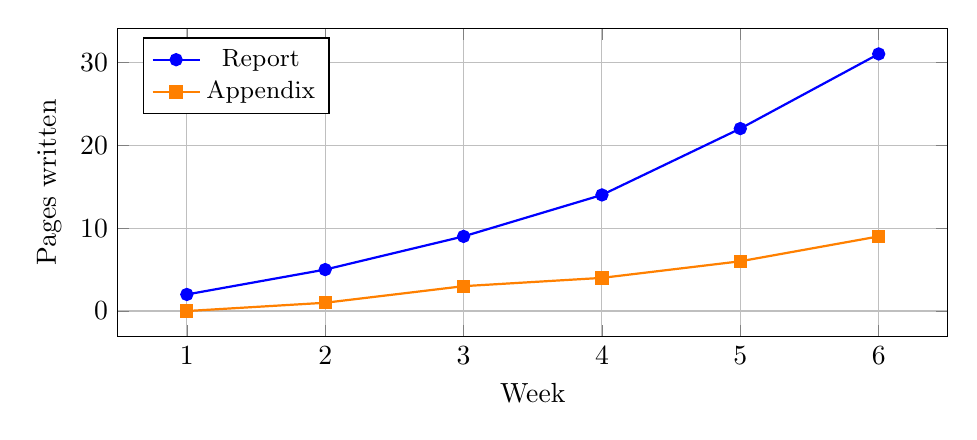
\begin{tikzpicture}
      \begin{axis}[
          width=\linewidth, height=5.5cm,
          xlabel={Week}, ylabel={Pages written},
          grid=major, legend pos=north west, legend style={font=\small}]
        \addplot[blue, thick, mark=*] coordinates {(1,2) (2,5) (3,9) (4,14) (5,22) (6,31)};
        \addlegendentry{Report}
        \addplot[orange, thick, mark=square*] coordinates {(1,0) (2,1) (3,3) (4,4) (5,6) (6,9)};
        \addlegendentry{Appendix}
      \end{axis}
    \end{tikzpicture}
    \caption{Line chart.}
    \label{fig:line-chart}
  \end{subfigure}
  \hfill
  \begin{subfigure}[b]{0.49\linewidth}
    \centering
    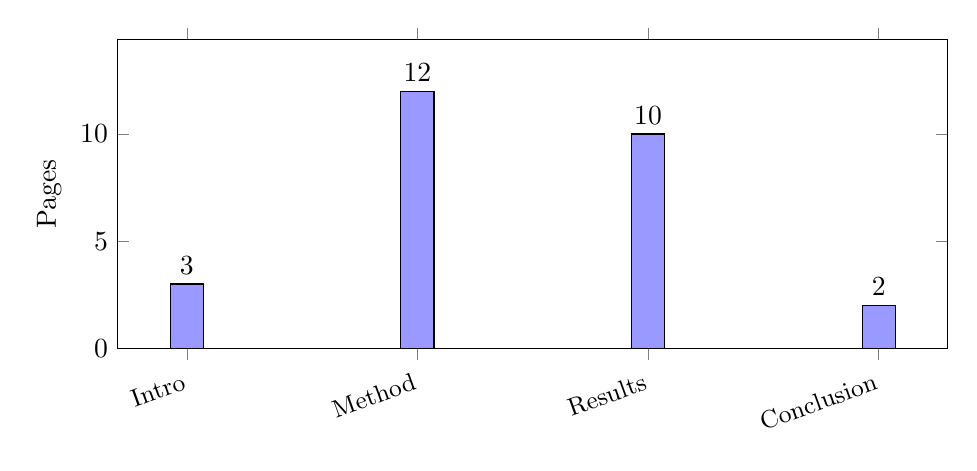
\begin{tikzpicture}
      \begin{axis}[
          width=\linewidth, height=5.5cm,
          ybar, bar width=12pt, ymin=0,
          symbolic x coords={Intro, Method, Results, Conclusion},
          xtick=data, x tick label style={font=\small, rotate=20, anchor=north east},
          ylabel={Pages}, nodes near coords, enlarge y limits={upper, value=0.2}]
        \addplot[fill=blue!40] coordinates {(Intro,3) (Method,12) (Results,10) (Conclusion,2)};
      \end{axis}
    \end{tikzpicture}
    \caption{Bar chart.}
    \label{fig:bar-chart}
  \end{subfigure}
  \caption{Charts drawn with PGFPlots.}
  \label{fig:charts}
\end{figure}
